%%%%%%%%%%%%%%%%%%%%%%%%%%%%%%%%%%%%%%%%%
% University/School Laboratory Report
% LaTeX Template
% Version 4.0 (March 21, 2022)
%
% This template originates from:
% https://www.LaTeXTemplates.com
%
% Authors:
% Vel (vel@latextemplates.com)
% Linux and Unix Users Group at Virginia Tech Wiki
%
% License:
% CC BY-NC-SA 4.0 (https://creativecommons.org/licenses/by-nc-sa/4.0/)
%
%%%%%%%%%%%%%%%%%%%%%%%%%%%%%%%%%%%%%%%%%

%----------------------------------------------------------------------------------------
%	PACKAGES AND DOCUMENT CONFIGURATIONS
%----------------------------------------------------------------------------------------

\documentclass[
	letterpaper, % Paper size, specify a4paper (A4) or letterpaper (US letter)
	11pt, % Default font size, specify 10pt, 11pt or 12pt
]{CSUniSchoolLabReport}

\usepackage{subcaption}
\usepackage{booktabs}
\geometry{top=1cm} % Override top margin to reduce space before title

%----------------------------------------------------------------------------------------
%	REPORT INFORMATION
%----------------------------------------------------------------------------------------

\title{Lab 3 - Electric Potential} % Report title

\author{Yiran \textsc{Liu} \&  Zijin \textsc{Yang}} % Author name(s), add additional authors like: '\& James \textsc{Smith}'

%----------------------------------------------------------------------------------------

\begin{document}

\maketitle % Insert the title, author and date using the information specified above

\begin{center}
	\begin{tabular}{l r}
      Course: & ECE 106 \\
      Student Number: & Y.L. 21184901 \& Z.Y. 21196273
	\end{tabular}
\end{center}
%----------------------------------------------------------------------------------------
%	COMPUTATIONS
%----------------------------------------------------------------------------------------

\section{Simulation}

We create the simulation in COMSOL for charged circular metal plates with radius $r=0.1m$ and separation distance:
\[
    \{5mm, 10mm, 15mm, 20mm, 25mm, 30mm\}
\]

\begin{figure}[H] % [H] forces the figure to be placed exactly where it appears in the text
	\centering % Horizontally center the figure
	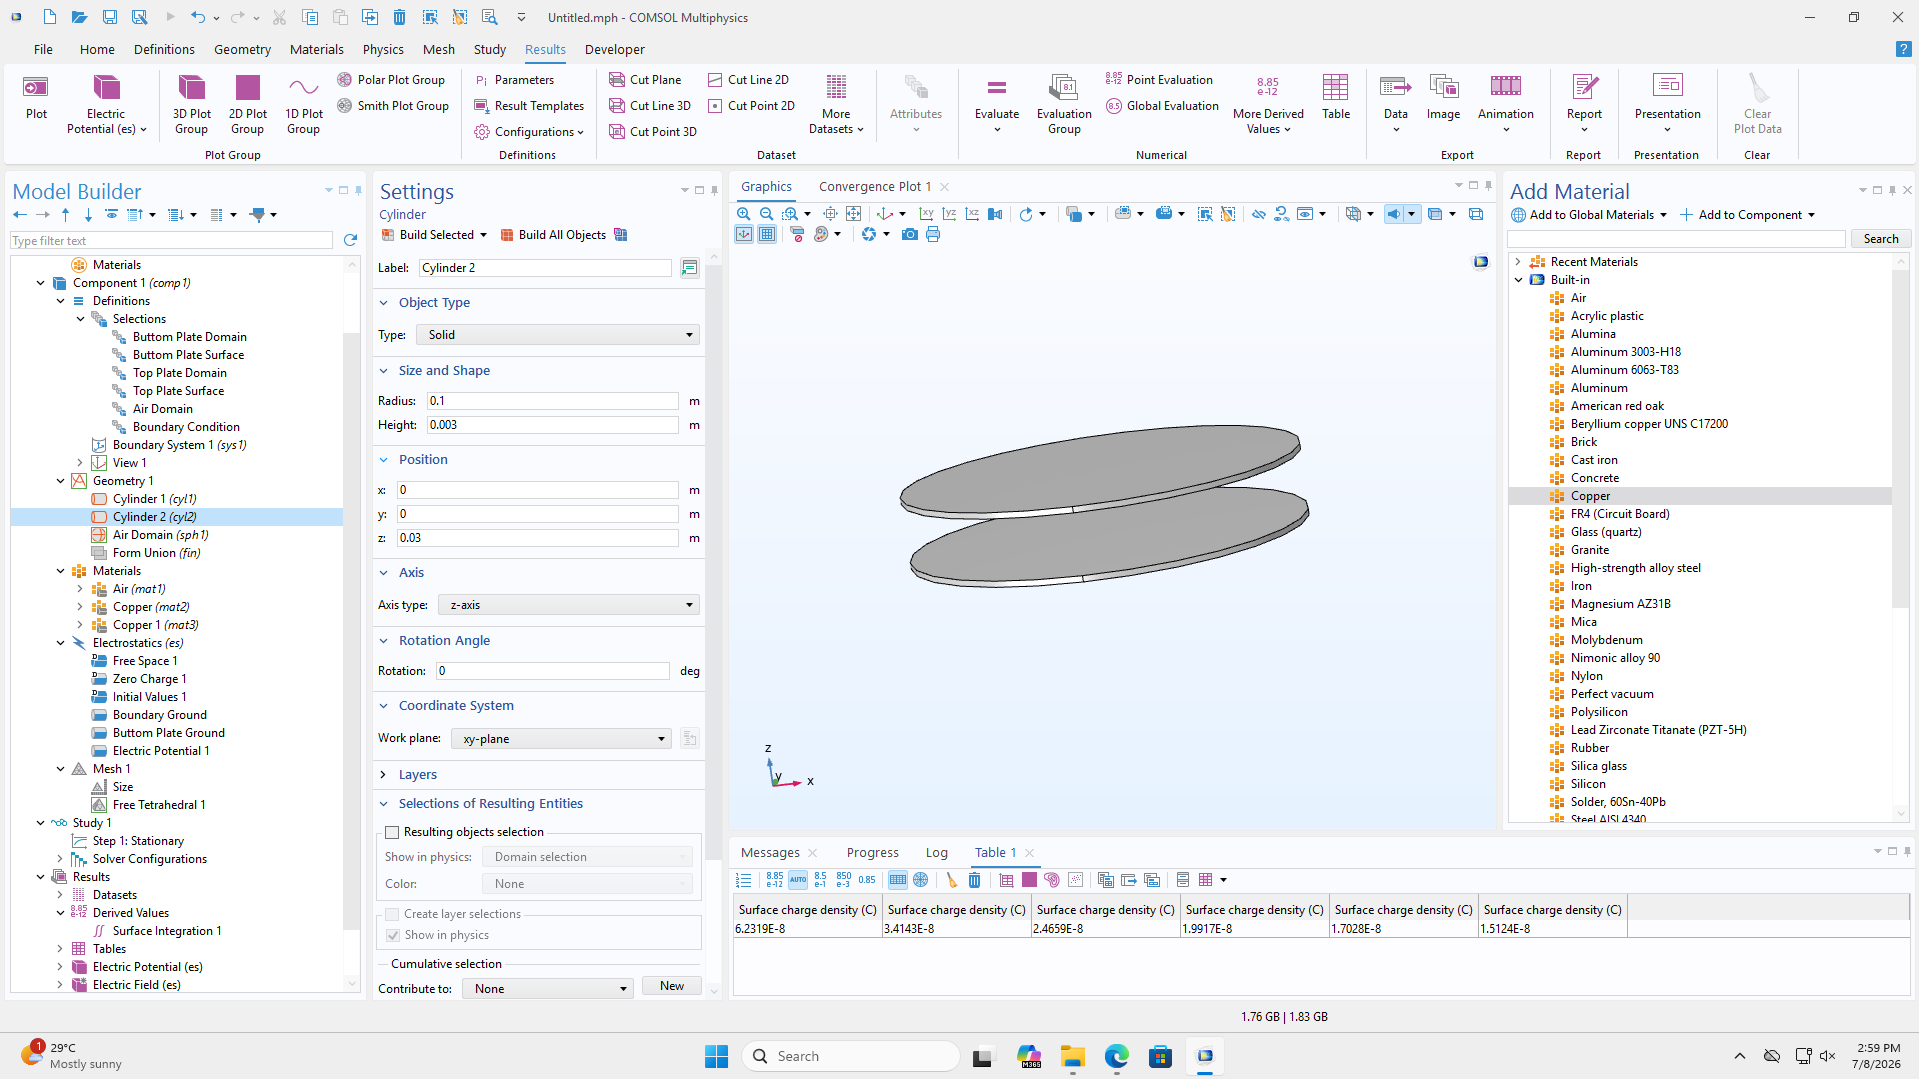
\includegraphics[width=1.0\textwidth]{./figures/Simulation30mm} % Include the figure
  \caption{Screenshot of COMSOL model and evaluated result (buttom-right).}
\end{figure}

We set voltage difference to be $\Delta V = 1000\text{V}$, and evaluated the total surface charge using surface integration $\iint_S dQ$.

\begin{table}[H]
    \centering
    \begin{tabular}{lcrr}
        \toprule
        \textbf{Separation ($mm$)} & \textbf{Surface Charge ($nC = 10^{-9}C$)} \\
        \midrule
        $5$  & $62.319$ \\
        $10$ & $34.143$ \\
        $15$ & $24.659$ \\
        $20$ & $19.917$ \\
        $25$ & $17.028$ \\
        $30$ & $15.124$ \\
        \bottomrule
    \end{tabular}
\end{table}


\section{Comparison of Results}

\subsection{Theoretical Computation}

We evaluated the theoretical result using the equation
\[
    C = \frac{\epsilon_0 A}{d}, \quad A = \pi r^2 = 0.0314159 m^2 
\]
this implies the following assumptions:

\begin{itemize}
    \item Excessive charge on the surface is considered to be distributed evenly.
    \item Size of the plate is large enough compared to the separation that the electric field in the space between can be considered even. 
    \label{assumptions}
\end{itemize}

\subsection{Simulation}
We compute the capacitance of the simulation model using: 
\[
    C = \frac{Q}{\Delta V}, \quad \text{where } \Delta V = 1000 \text{V}
\]

\subsection{Lab Measurement}

We measure the capacitance between the plates when they are separated by a large distance as $C_\text{null}$ and subtract it from our results.

\subsection{Table \& Graph}

\begin{figure}[H] % [H] forces the figure to be placed exactly where it appears in the text
	\centering % Horizontally center the figure
	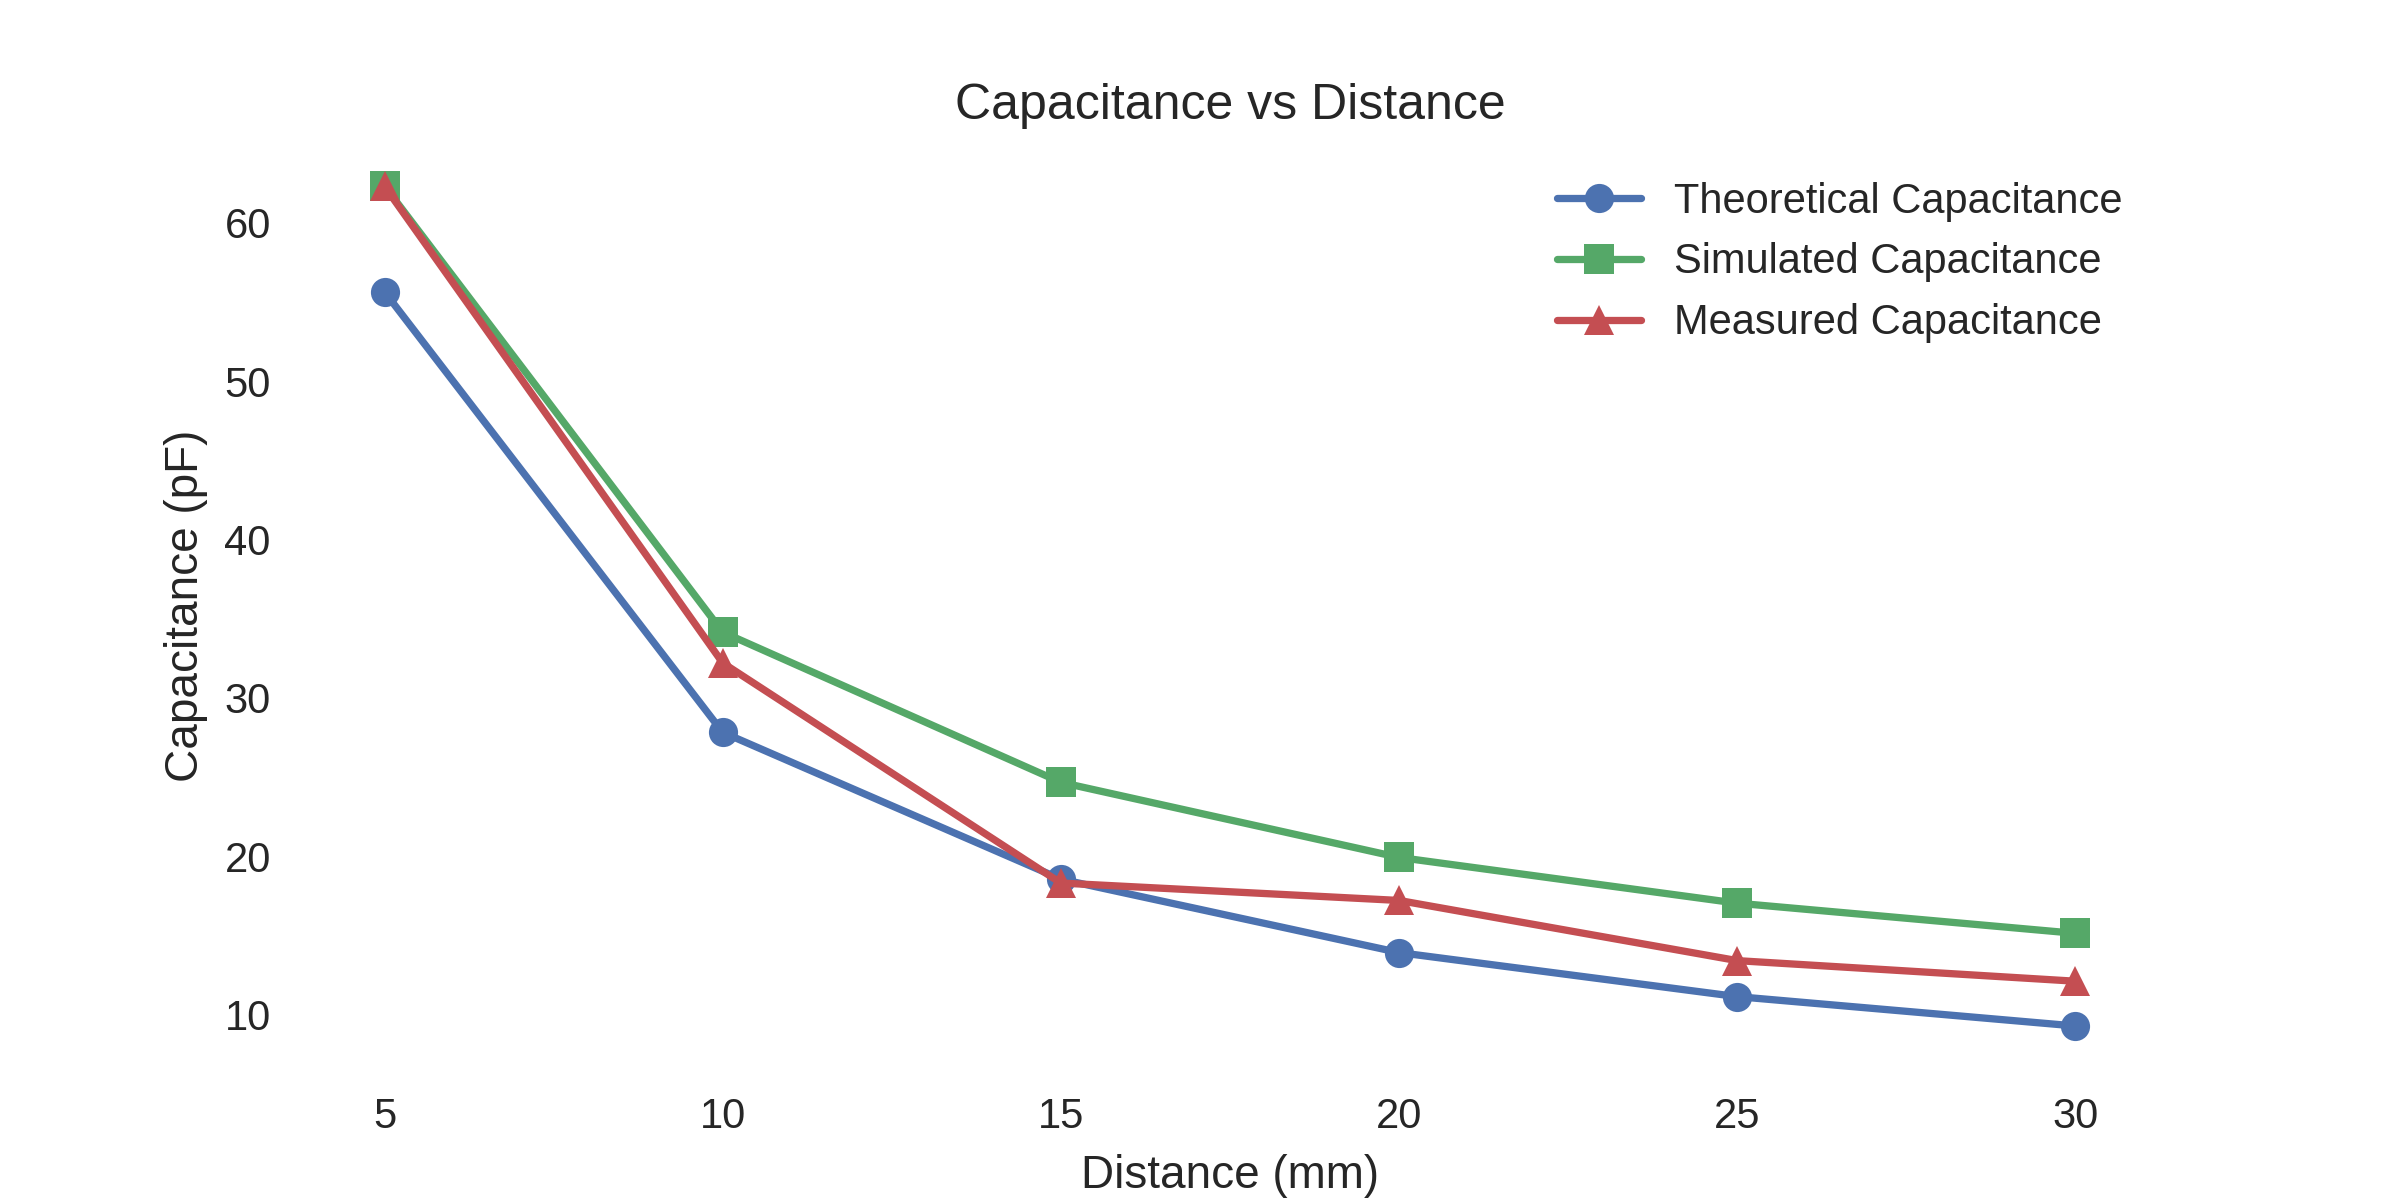
\includegraphics[width=1.0\textwidth]{./figures/capacitance_vs_distance} % Include the figure
\end{figure}

\begin{table}[H]
    \centering
    \begin{tabular}{lcrr}
        \toprule
        \textbf{Separation ($mm$)} & \textbf{Theoretical} & \textbf{Simulated} & \textbf{Measured ($pF$)} \\
        \midrule
        5  & 55.6325 & 62.319 & 62.3 \\
        10 & 27.8163 & 34.143 & 32.2 \\
        15 & 18.5442 & 24.659 & 18.3 \\
        20 & 13.9081 & 19.917 & 17.2 \\
        25 & 11.1265 & 17.028 & 13.4 \\
        30 & 9.27208 & 15.124 & 12.1 \\
        \bottomrule
    \end{tabular}
\end{table}

\section{Discussion}

\subsection{Theoretical Error Source}

The two most significant sources of error are exactly the two assumptions we made. In reality:

\begin{itemize}
    \item Excessive charge on the surface is \textbf{not} distributed evenly.
    \item The electric field in the space between is \textbf{not} even. 
\end{itemize}

We can confirm this by plotting the surface charge density in the simulation result:

\begin{figure}[H] % [H] forces the figure to be placed exactly where it appears in the text
    \centering % Horizontally center the figure
    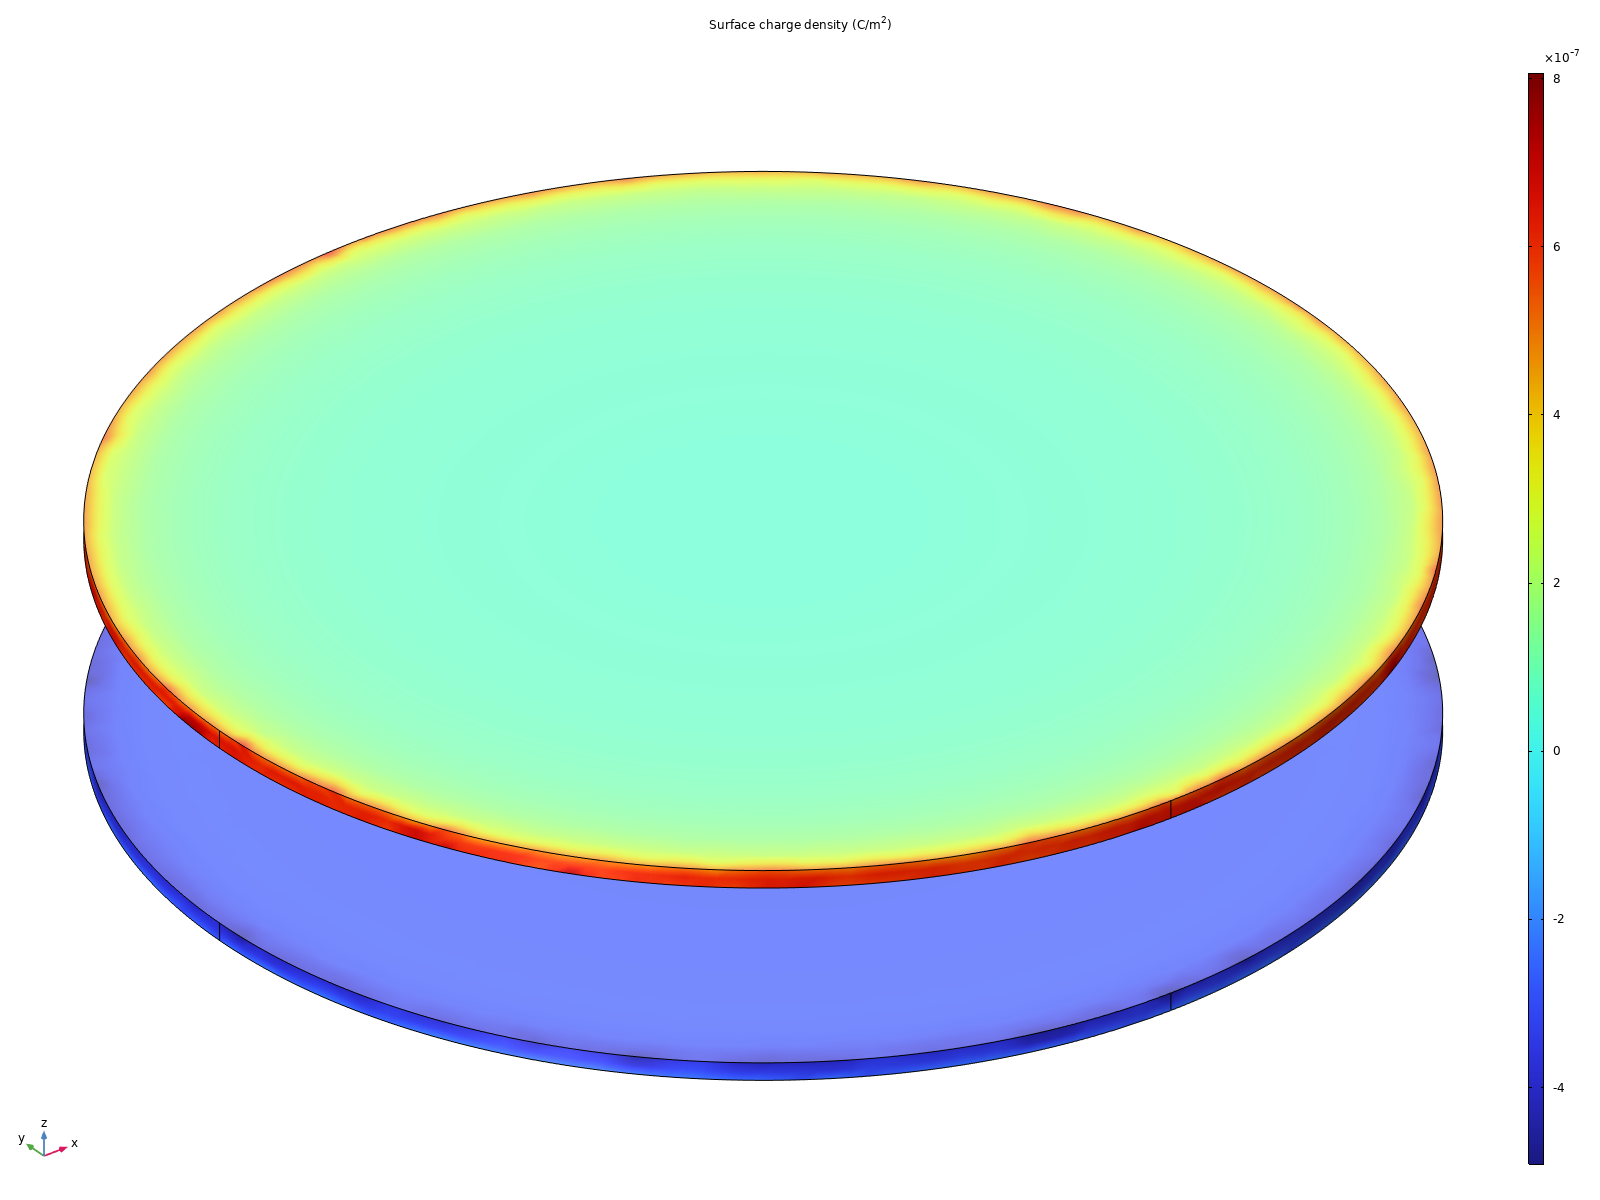
\includegraphics[width=0.6\textwidth]{figures/ChargeDensity.png} % Include the figure
    \caption{Surface charge density in the COMSOL model; the area around the edge has a significantly higher density.}
\end{figure}



\subsection{Simulation Error Source}

The two most significant sources of error are:

\begin{itemize}
    \item FEM's fundamental constraint of element size, especially around edges of the plate where energy density changes rapidly
    \item Boundary condition assumes pure air around device
\end{itemize}

\subsection{Measurement Error Source}

The two most significant sources of error are:

\begin{itemize}
    \item The plates are not exactly parallel.
    \item Imperfect wire and instrument, and other environmental disturbances
\end{itemize}

\subsection{Engineering Design Decision}


To approximate the \textbf{expected} (mean) capacitance of the device, I will use the \textbf{COMSOL Simulation} result, since it has the least significant error sources and correctly accounts for the uneven charge distribution.

However, to find a \textbf{safe range} of the capacitance for safety critical applications, I will choose \textbf{real-life measurement}. We will need to measure multiple samples from a batch of manufactured parts and compute the mean and standard deviation. Then, derive a range-of-tolerance (e.g., $\pm 15\%$).

\pagebreak

\section{Challenge Activity}

\subsection{Experiment Set-up}

We will measure the dielectric constant $\epsilon_r$ of dielectric plates -- one circular and one semi-circular -- by measuring the electric capacitance between the two conducting plates, using the experiment set-up below:

\begin{figure}[H]
    \centering
    % First image (Experiment Setup)
    \begin{subfigure}{0.4\textwidth} % 0.48 to leave a small gap between images
        \centering
        % \textwidth here is relative to the subfigure's width (0.48), not the whole page
        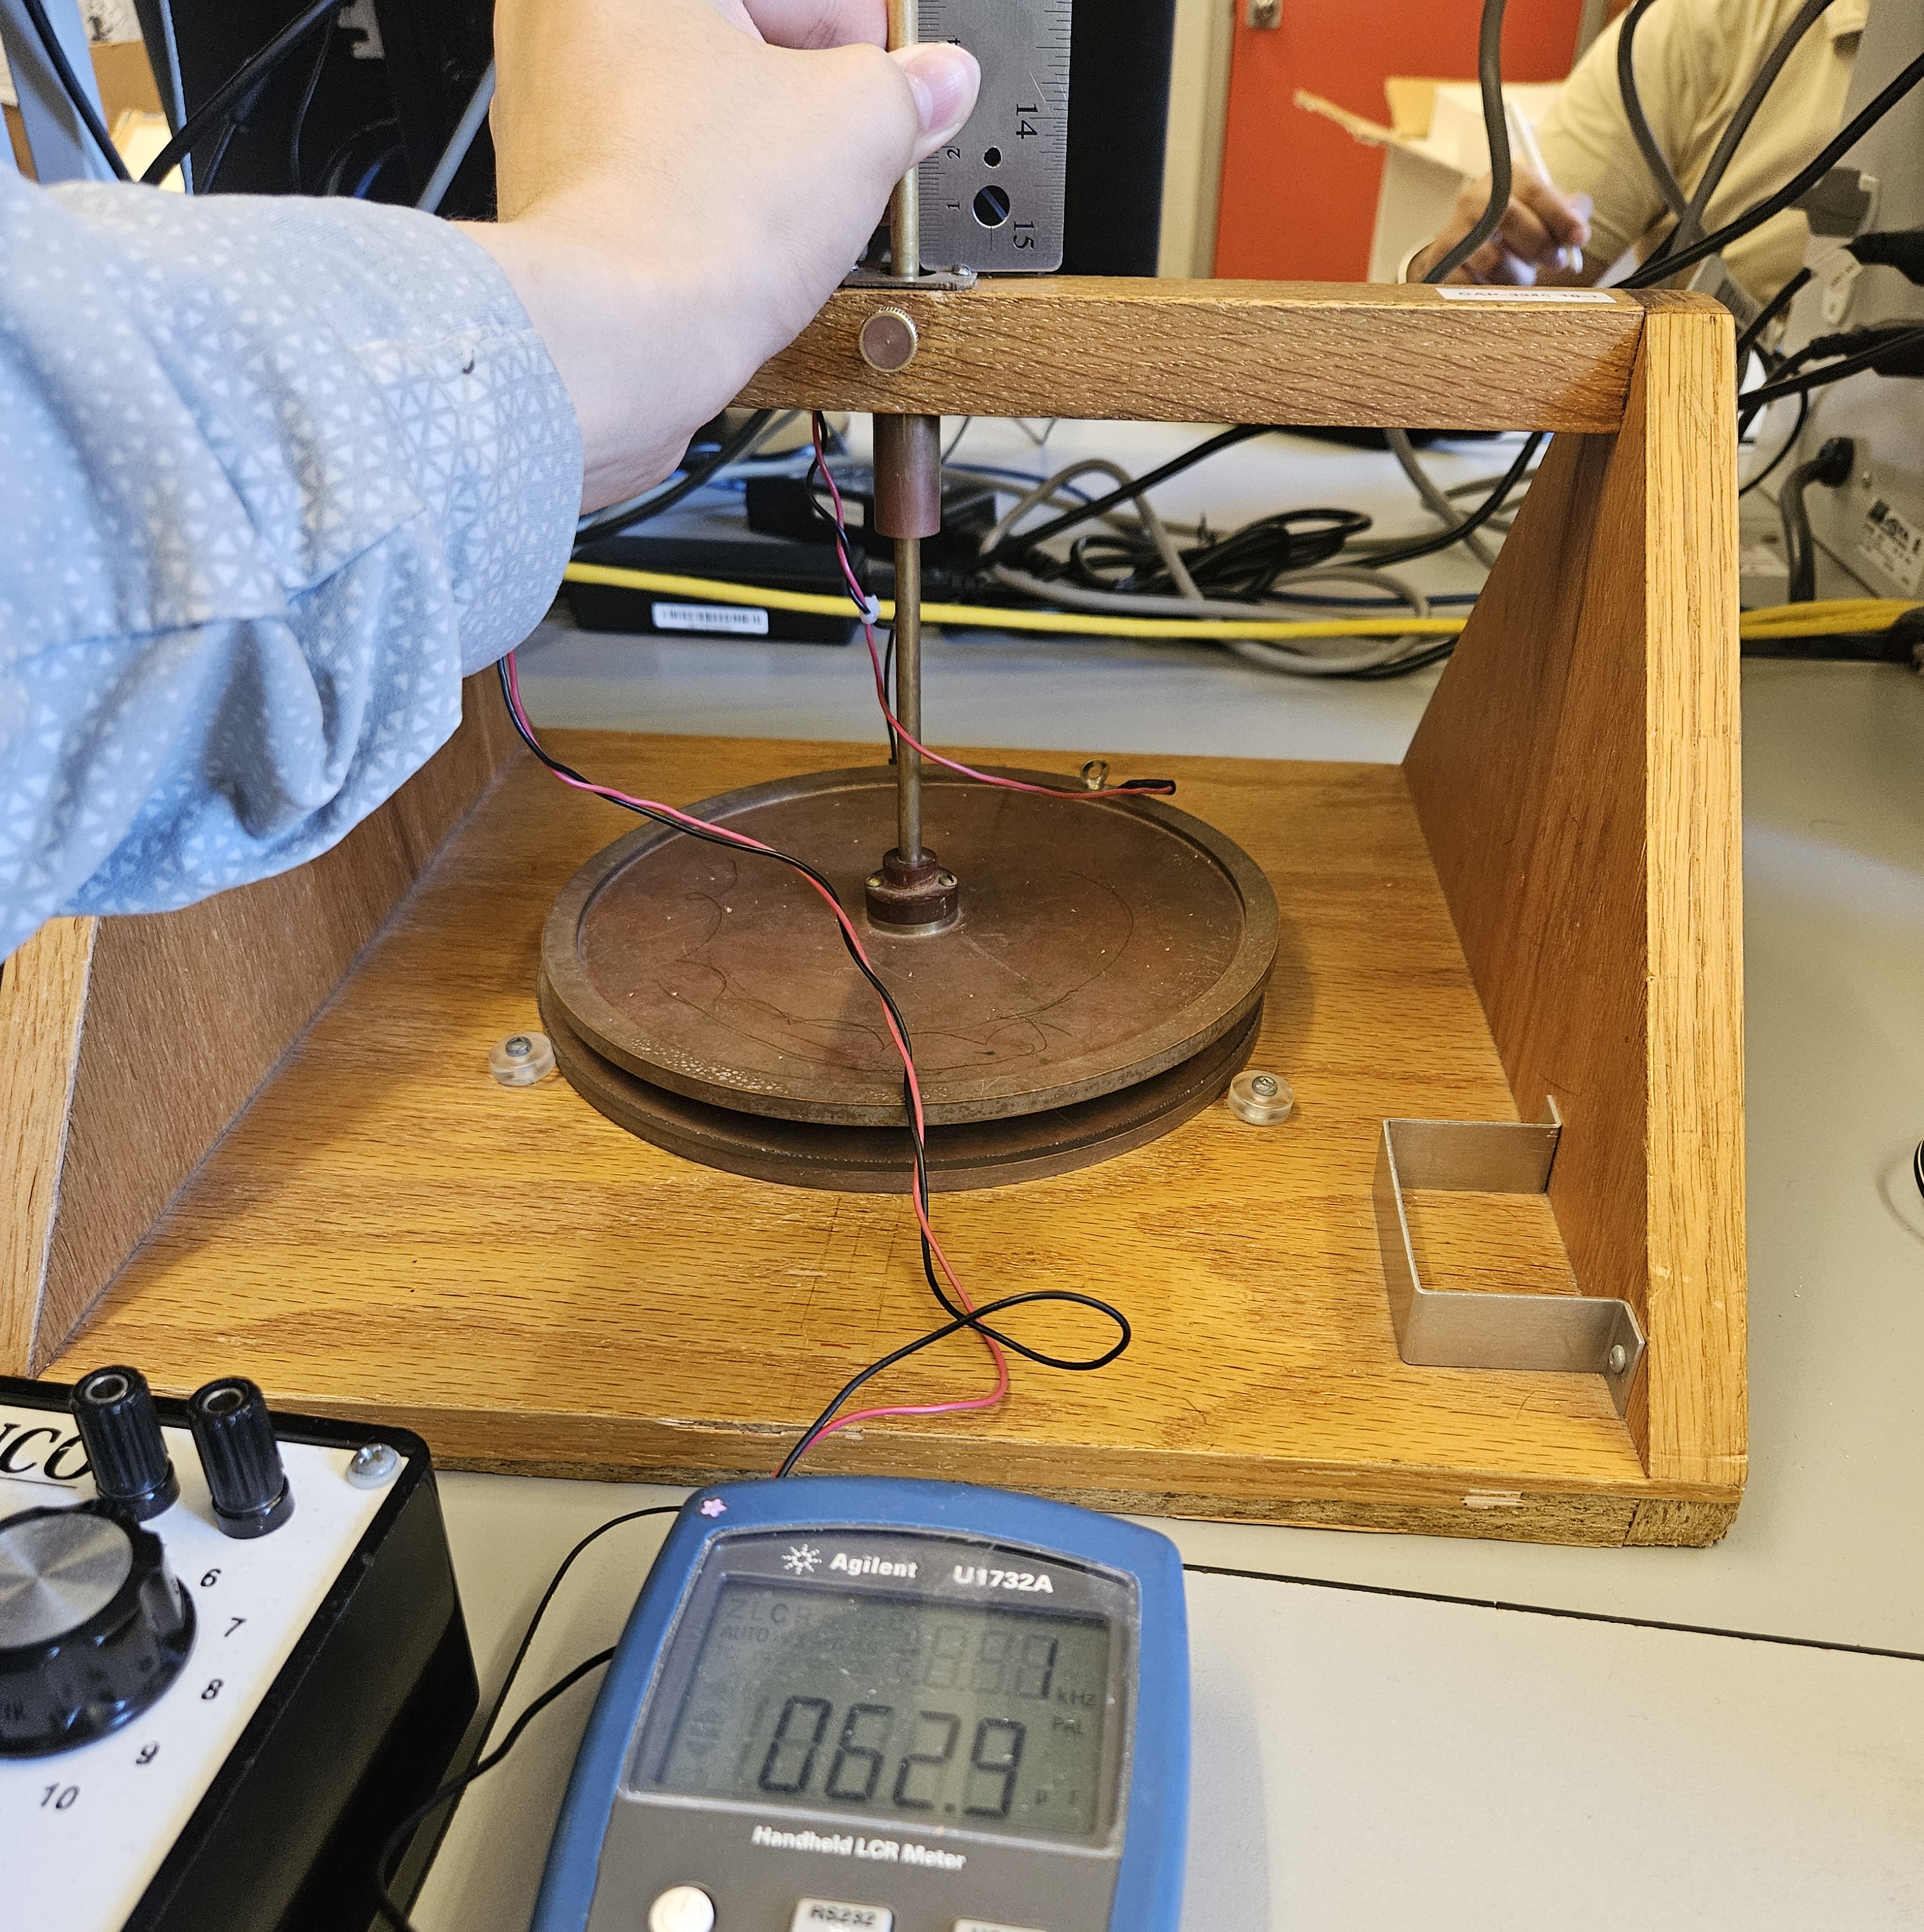
\includegraphics[width=\textwidth]{figures/setup.jpg} 
    \end{subfigure}\hfill % \hfill pushes the images apart horizontally
    %
    % Second image (Dielectric samples)
    \begin{subfigure}{0.4\textwidth}
        \centering
        % Replace "DielectricPhoto" with your actual file name
        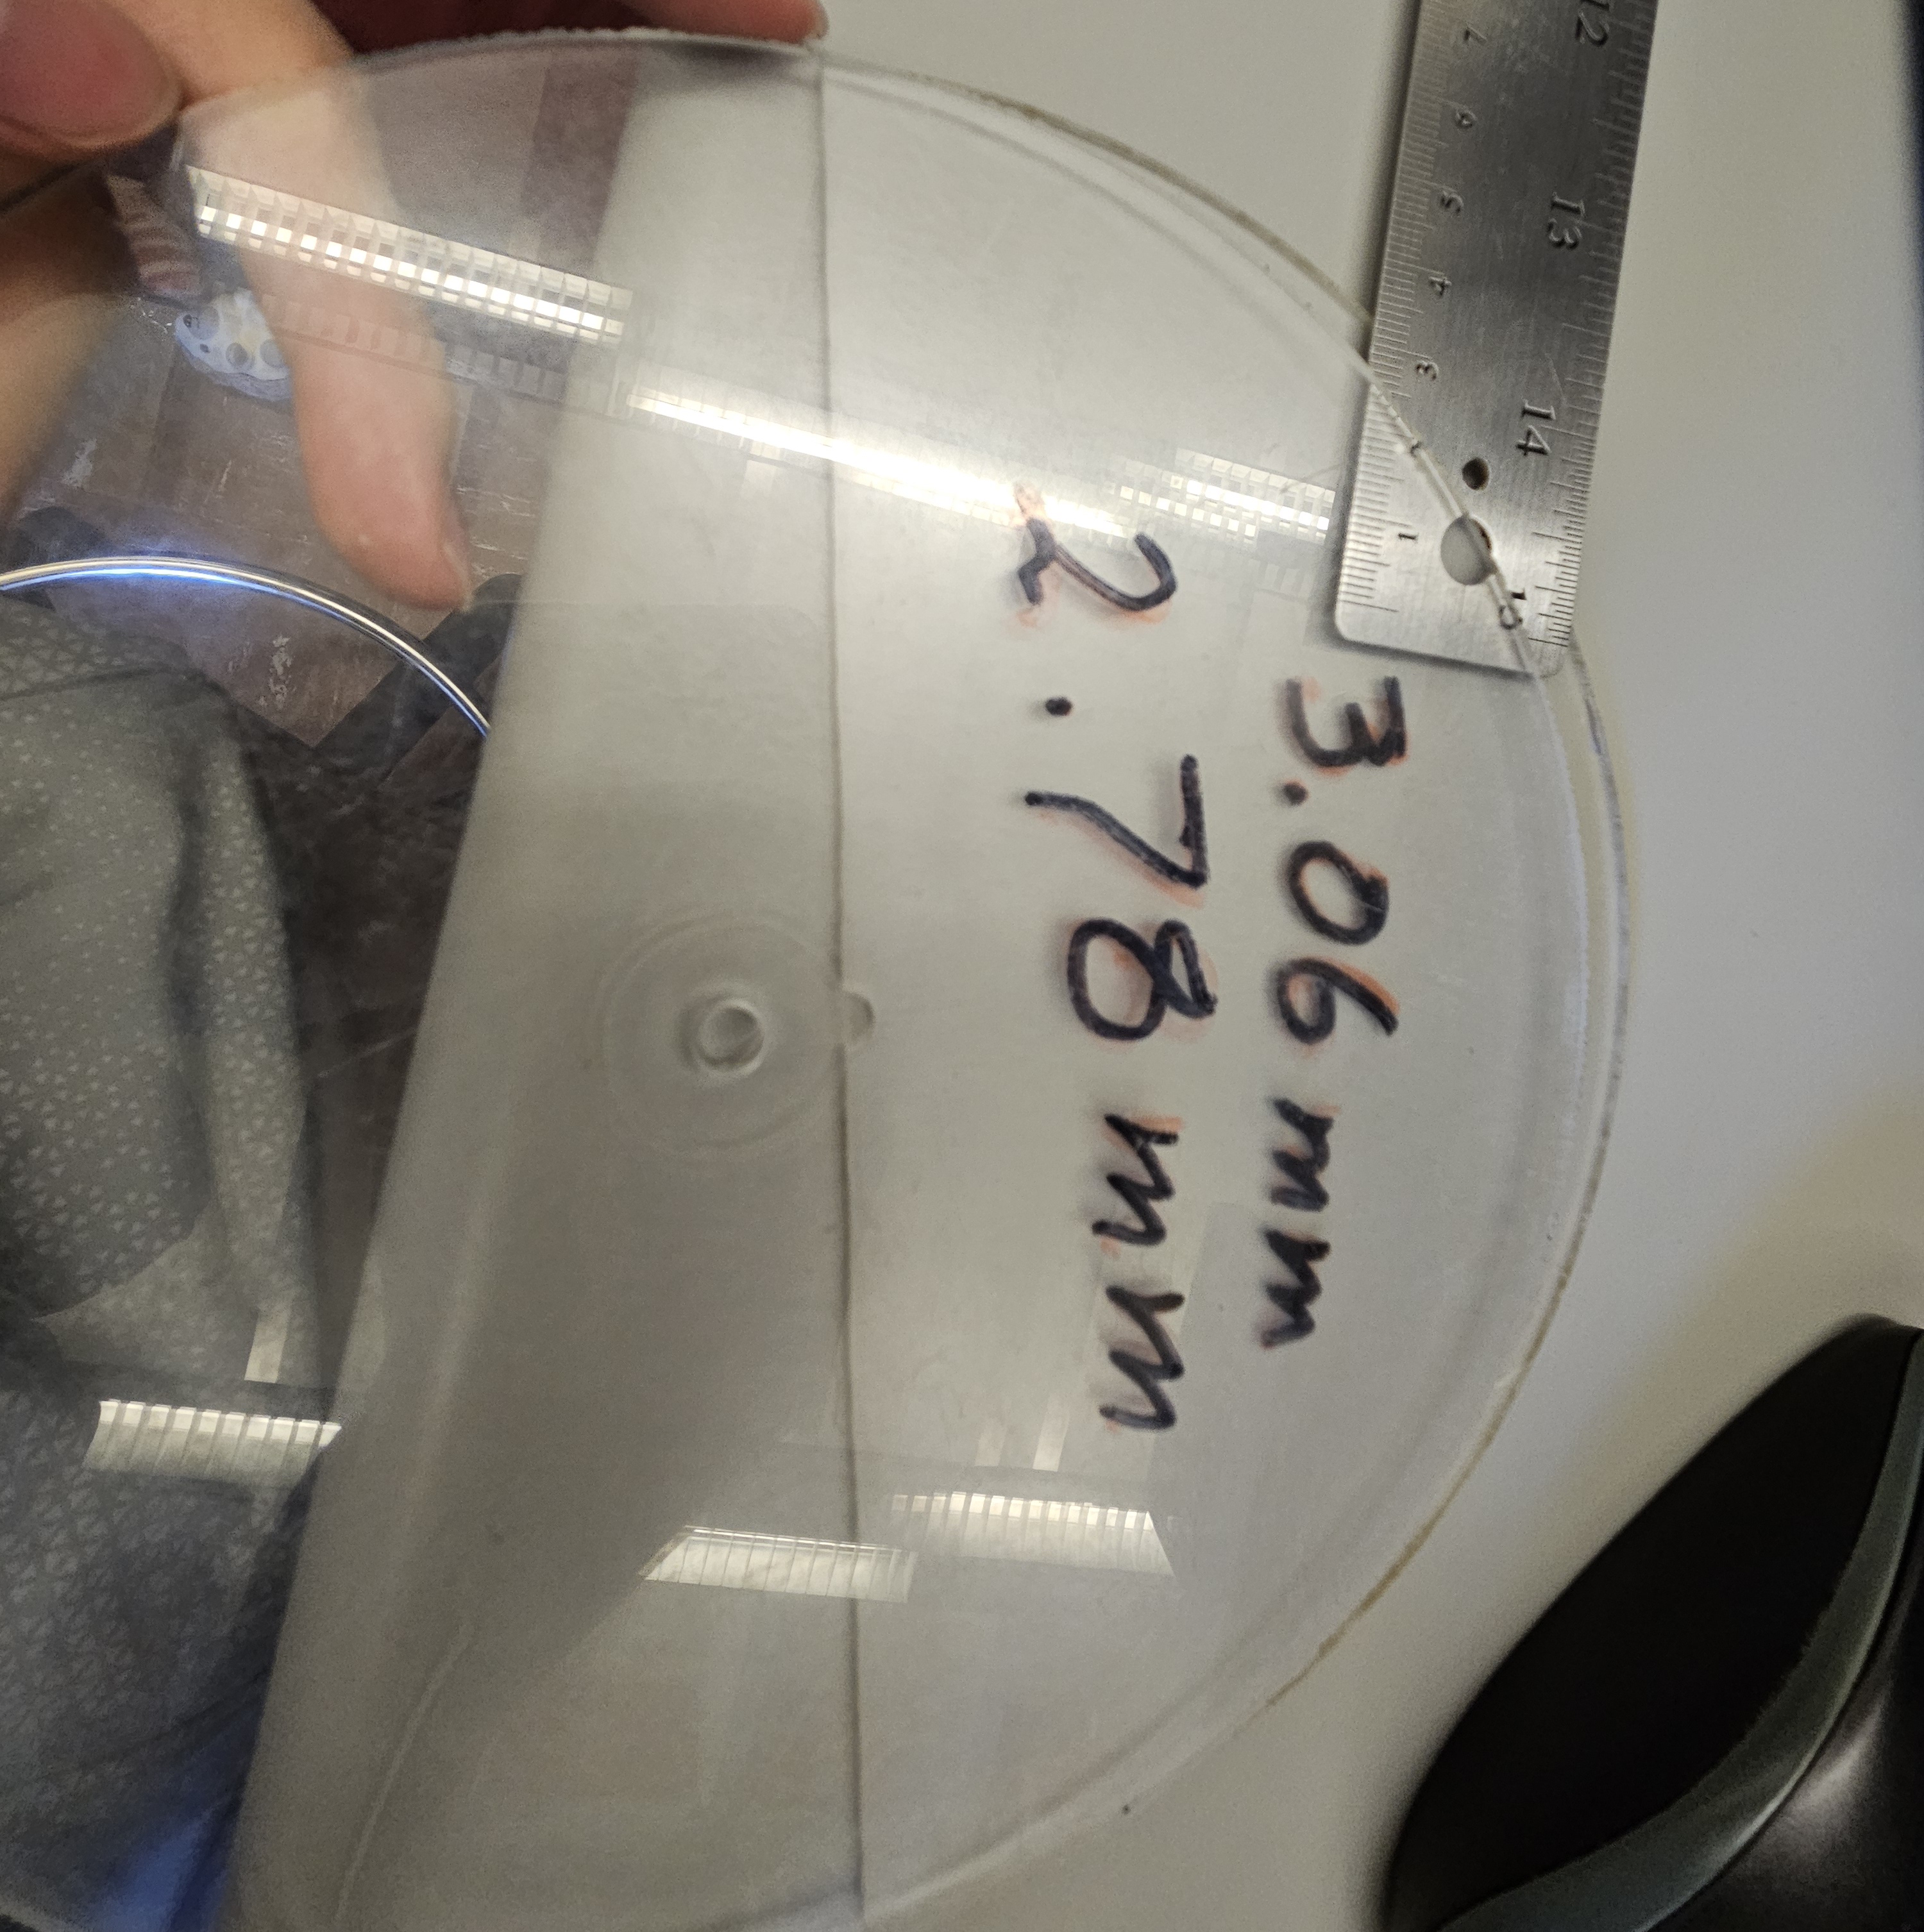
\includegraphics[width=\textwidth]{figures/dieletric.jpg}
    \end{subfigure}

    \caption{Photos of the experiment setup (left) and dielectric plates (right).}
    \label{fig:challenge_photos}
\end{figure}

\subsection{Physics Model}

\begin{figure}[H] % [H] forces the figure to be placed exactly where it appears in the text
	\centering % Horizontally center the figure
	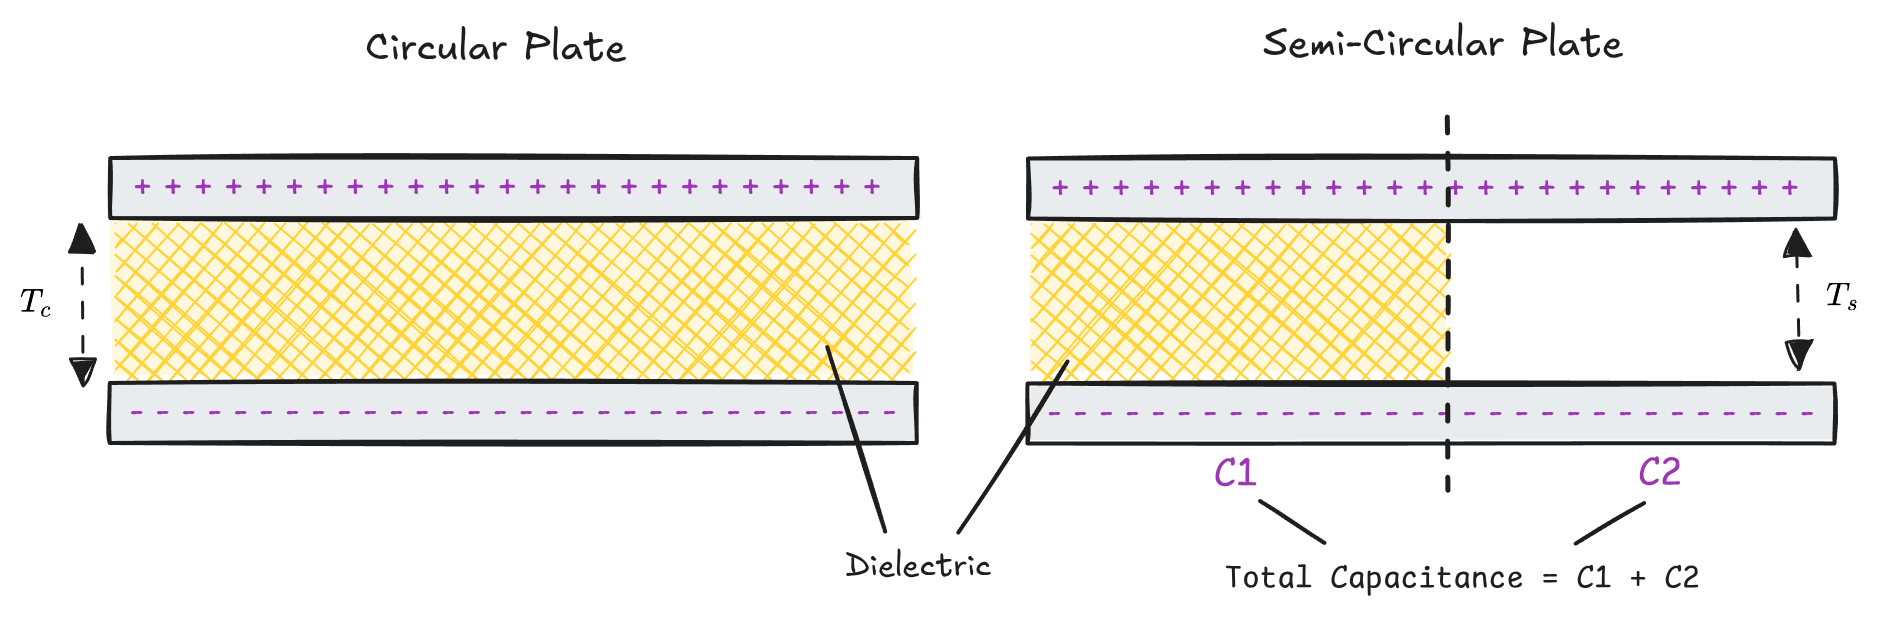
\includegraphics[width=0.8\textwidth]{./figures/Model.png} % Include the figure
  \caption{}
\end{figure}

We consider the two models, the capacitance of the circular dielectric $C_c$ and that of the semi-circular di-electric $C_s$ are:
\[
    C_c = \frac{\epsilon_0 \epsilon_r A}{T_c} \quad\quad C_s = \frac{\epsilon_0 \epsilon_r A}{2 T_s} + \frac{\epsilon_0 A}{2 T_s}
\]

\[
    C_s / C_c = \frac{\epsilon_r + 1}{2T_s} / \frac{\epsilon_r}{T_c} = \frac{T_c}{2T_s} \frac{\epsilon_r + 1}{\epsilon_r} \implies \frac{\epsilon_r +1}{\epsilon_r} = \frac{2C_s T_s}{C_c T_c}
\]

\subsection{Computation}

\begin{table}[H]
    \centering
    \begin{tabular}{lcrr}
        \toprule
        \textbf{Capacitance}\tiny{ Semi-circle} & \textbf{Capacitance}\tiny{ Circle} & \textbf{Thickness}\tiny{ Semi-circle} & \textbf{Thickness}\tiny{ Circle} \\
        \midrule
        183.5pF & 270.1pF & 2.78mm & 3.06mm \\
        \bottomrule
    \end{tabular}
\end{table}

\[
    \boxed{\epsilon_r = 4.26575}
\]
\end{document}